\documentclass[addpoints]{exam}

\usepackage{graphbox}
\usepackage{hyperref}
\usepackage{tabularx}
\usepackage{tikz}
\usetikzlibrary{positioning}

% Header and footer.
\pagestyle{headandfoot}
\runningheadrule
\runningfootrule
\runningheader{CS 440 Computer Graphics}{Homework 1}{Spring 2018}
\runningfooter{}{Page \thepage\ of \numpages}{}
\firstpageheader{}{}{}

\qformat{{\large\bf \thequestion. \thequestiontitle}\hfill[\totalpoints\ points]}
\boxedpoints
% \printanswers

\title{Habib University\\CS 440 Computer Graphics\\Spring 2018}
\author{Homework 1}
\date{Due: TBD}

\begin{document}
\maketitle

\begin{questions}

  \titledquestion{Mapping and Linear Interpolation}[5]
  \begin{tabularx}{\textwidth}{cX}
    \raisebox{-\totalheight}{
      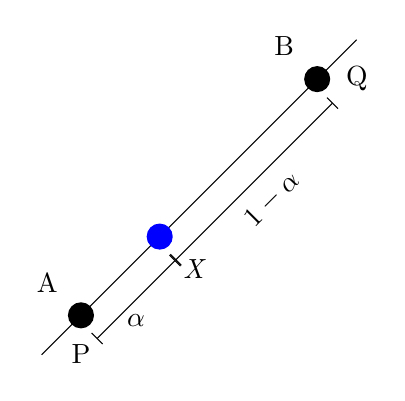
\begin{tikzpicture}
        \draw (0,0) -- (4,4);
        \node[circle,fill] at (.5,.5) (P){};
        \node[circle,fill] at (3.5,3.5) (Q) {};
        \node[circle,fill,blue] at (1.5,1.5) (X) {};
        \node[below  = 2pt of P]{P};
        \node[right = 2pt of Q]{Q};
        \node[below right = 2pt of X]{\it X};
        \node[above left = 2pt of P]{A};
        \node[above left = 2pt of Q]{B};

        \draw[|-|] (0.7,0.2) -- node[midway,below=2pt]{$\alpha$}(1.7,1.2);
        \draw[|-|] (1.7,1.2) -- node[midway,sloped,below=2pt]{$1-\alpha$}(3.7,3.2);
      \end{tikzpicture}
    }
    &
    For any point $X$ on the line segment PQ, the distance of $R$ to the endpoints can be expressed as
    \[
      |PX| : |XQ| = \alpha:(1-\alpha)\;,\; 0 \leq \alpha \leq 1
    \]
    which leads to
    \[
      X = \alpha Q + (1-\alpha) P
    \]
    $X$ is thus said to be an \href{https://en.wikipedia.org/wiki/Affine_combination}{\it affine combination} of P and Q.
    
    Imagine a mapping from the range PQ to a new range, AB. We are interested in findining the coordinates of $X'$ which is the mapping of $X$ to the new range. Write a function {\tt map\_point(px, py, qx, qy, ax, ay, bx, by, x, y, \&\_x, \&\_y)} that takes as argument the coordinates of P, Q, A, B, and X and sets the last 2 arguments to the coorindates of $X'$.
  \end{tabularx}
  
  \titledquestion{Interaction: Polygons Galore!}[20]
  
  \begin{tabularx}{\textwidth}{lX}
    \raisebox{-.85\totalheight}{\includegraphics[width=.4\textwidth]{galore}}
    &
    Write a program that interactively draws triangles and quadrilaterals. The program draws a point at the location of each mouse click. It supports two {\it modes} -- triangle mode (default) and quad mode. When in triangle mode, every 3 consecutive points are drawn as a triangle. When in quad mode, every 4 consecutive points are drawn as a quad.

    Furthermore, the following interaction is supported.\newline
    -- Pressing q or Q closes the window and ends the program.\newline
    -- Pressing r or R clears the screen and resets to default.\newline
    -- Pressing t or T toggles between the drawing modes.
  \end{tabularx}

  \titledquestion{Vertex Arrays}[10]

  \titledquestion{Idle Time: Catch me if you can}[20]
  Draw a 2D object with non-zero area anywhere on the screen. After a random interval of time, it automatically changes position. You have to try to click on the object. If you succeed, you gain a point, otherwise you lose a point. Once you reach -3 points, the game ends.

  Use: idle callback

  \titledquestion{Approximating Smooth Surfaces}[20]
  Approximate a circle using increasing number of points.

  \titledquestion{Color Interpolation: In memory of Tim}[5]
  Draw Maxwell's triangle.

  \titledquestion{Color Interpolation}[10]
  Draw the color bar.

  \titledquestion{Triangle in a Triangle in a Triangle ...}[20]
  Sierpinski gasket.

  \titledquestion{Deja Vu}[35]
  Mandelbrot set.


  
  
\end{questions}

\end{document}



